\section{Results}
\label{sec:results}

\subsection{Sensitivity}
 show impact of HM DY on PDFs using sensitivity studies based on
pseudo-data, for which we only use the data uncertainties, while central 
value are fixed:
 HERA I+II vs HERA I+II + HMDY --> see the sensitivity plots from the previous email

conclusion: HMDY data has a large impact on photonPDF 

\subsection{The photon PDF}

For the NNLO fit a $\chi^{2}/ndf = 1.18$, with a partial $\chi^2/ndp = 1.15$ for the high-mass Drell-yan data [{\it update with final numbers}], is achieved for the
parametrization described in the previous section.
%
Fig.~\ref{PDF_7.5GeV}
 shows the PDF distributions $x_{u_v},xd_{d_v},x\bar{u}, x\bar{d}, xg$ at $Q^{2}$ = 7.5$^{2}$ GeV$^{2}$,
including model and parametrisation uncertainties, while  Fig.~\ref{PDF_10000GeV} 
shows them at $Q^{2}$ = 10$^{4}$ GeV$^{2}$. {\it Add model and parametrisation variations, Use NNLO MC central}.
\begin{figure}
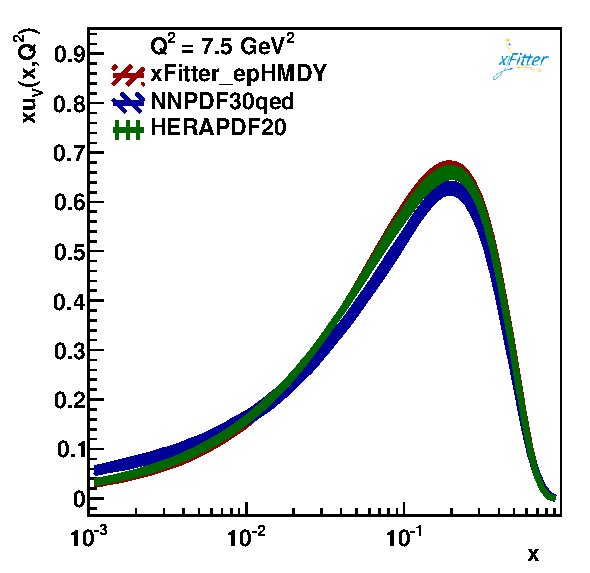
\includegraphics[width=7cm]{plots/uv_7_5.pdf} 
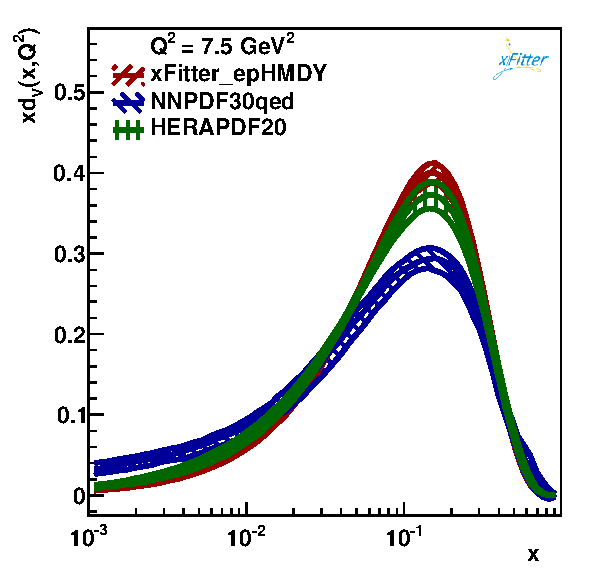
\includegraphics[width=7cm]{plots/dv_7_5.pdf} 
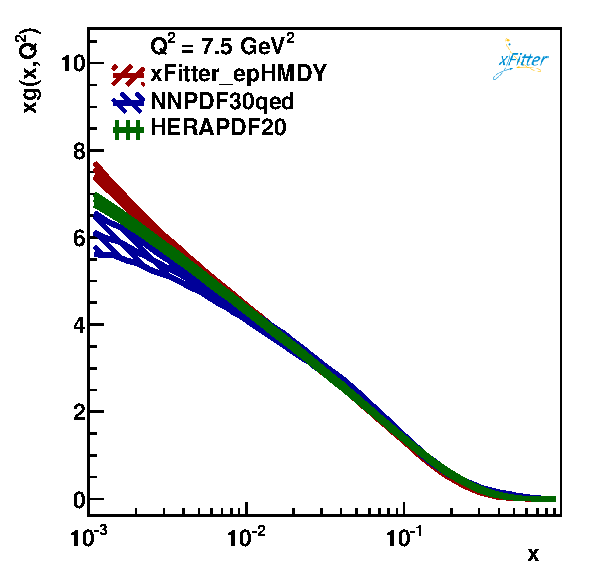
\includegraphics[width=7cm]{plots/gluon_7_5.pdf} 
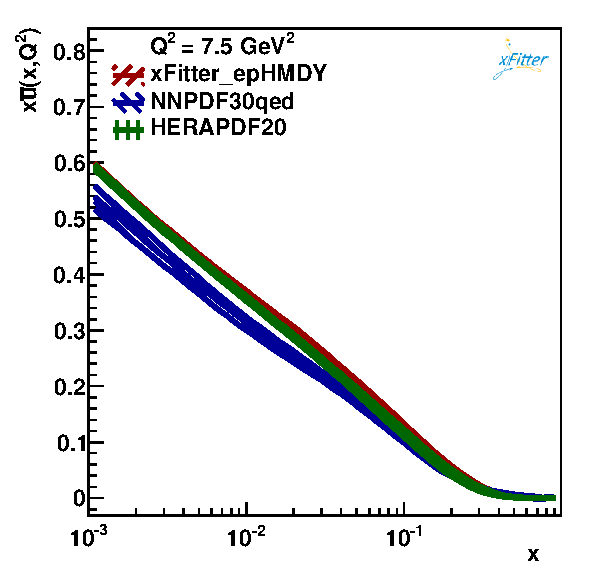
\includegraphics[width=7cm]{plots/ubar_7_5.pdf} 
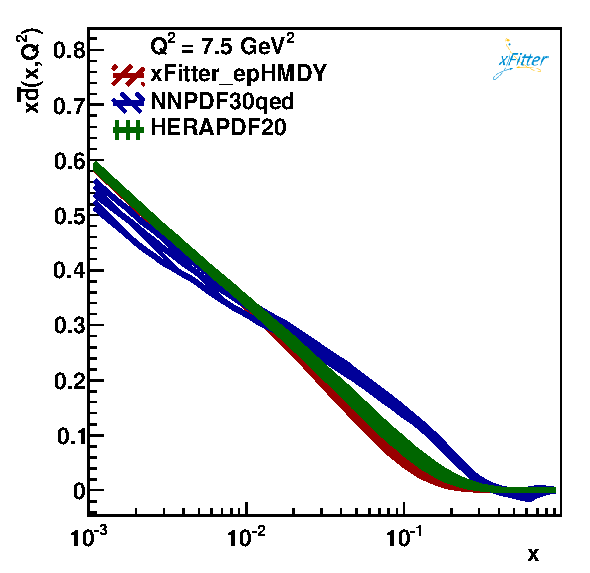
\includegraphics[width=7cm]{plots/dbar_7_5.pdf} 
\caption{NNLO PDF distributions at $Q^{2}$ = 7.5$^{2}$ GeV$^{2}$: (a) $u$ - valence; (b) $d$ - valence; (c) gluon; (d) $\bar{u}$; (e) $\bar{d}$ }
\label{PDF_7.5GeV}
\end{figure}
\begin{figure}
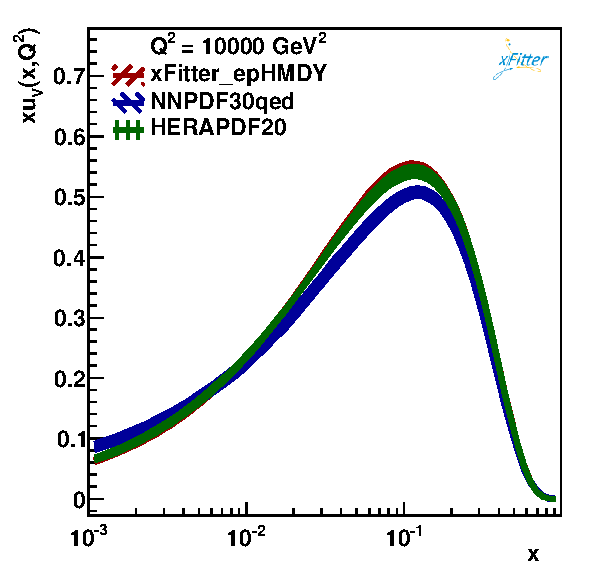
\includegraphics[width=7cm]{plots/uv_10000.pdf} 
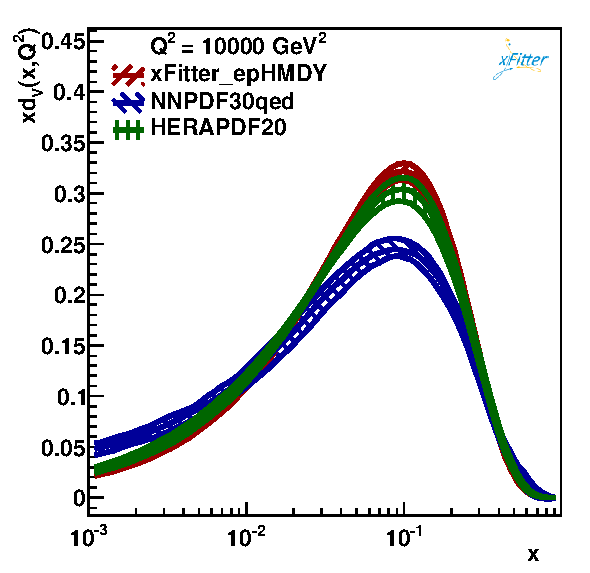
\includegraphics[width=7cm]{plots/dv_10000.pdf} 
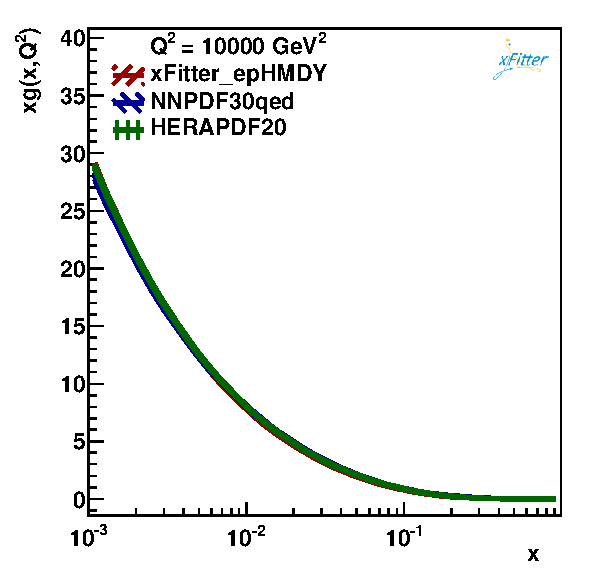
\includegraphics[width=7cm]{plots/gluon_10000.pdf} 
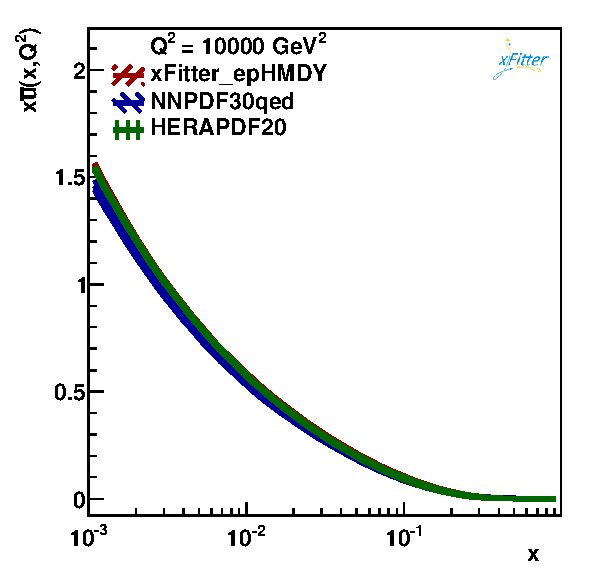
\includegraphics[width=7cm]{plots/ubar_10000.pdf} 
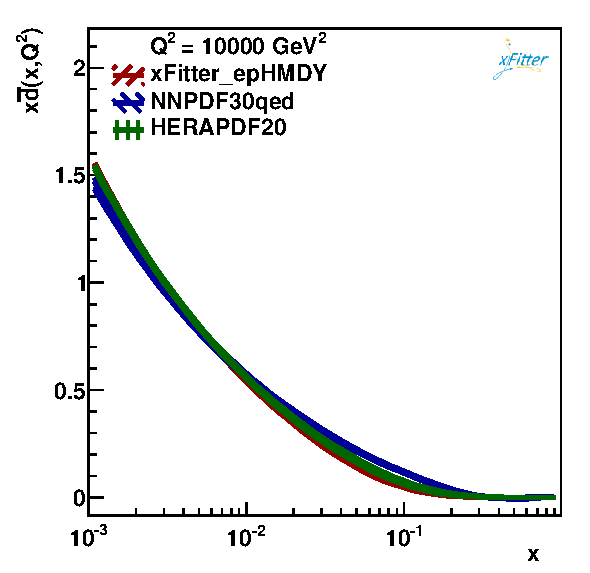
\includegraphics[width=7cm]{plots/dbar_10000.pdf} 
\caption{NNLO PDF distributions at $Q^{2}$ = 10000$^{2}$ GeV$^{2}$: (a) $u$ - valence; (b) $d$ - valence; (c) gluon; (d) $\bar{u}$; (e) $\bar{d}$}
\label{PDF_10000GeV}
\end{figure}
In these figures comparisons are made to the NNPDF3.0PDF set and the HERAPDF2.0 set.
The shape of the $xd_{u_v}$ distribution is close to that of HERAPDF2.0 
because of the dominance of HERA data in the fit. 


Fig.~\ref{hmDY_2D} 
shows the comparison between the high-mass Drell-Yan double differential distribution and 
the predictions.
\begin{figure}
\centering
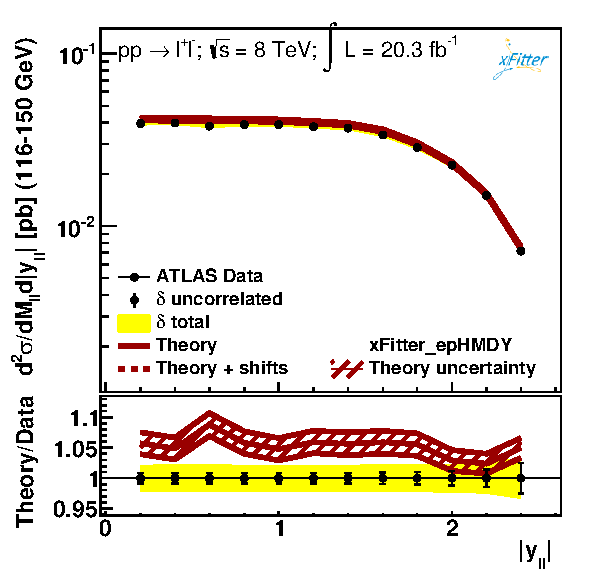
\includegraphics[width=7cm]{plots/data_1.pdf} 
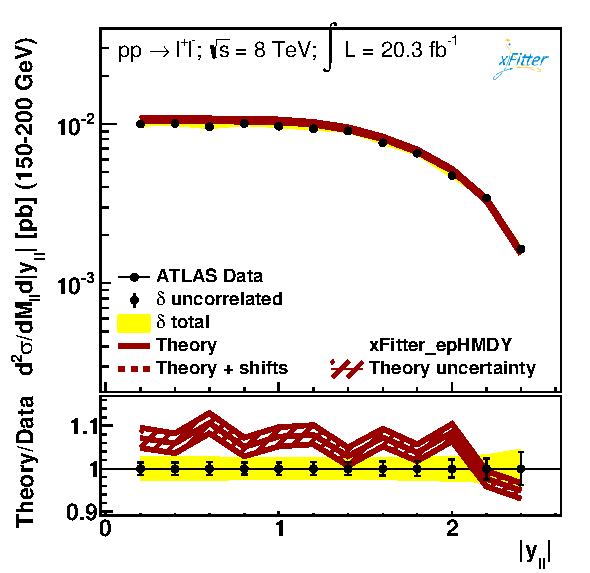
\includegraphics[width=7cm]{plots/data_2.pdf} 
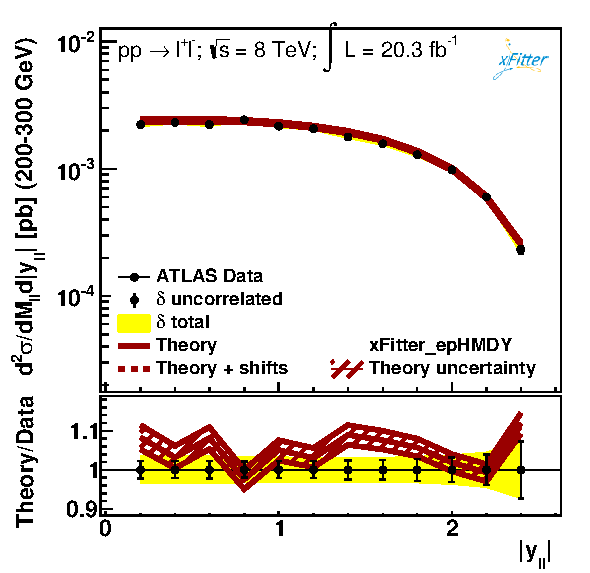
\includegraphics[width=7cm]{plots/data_3.pdf} 
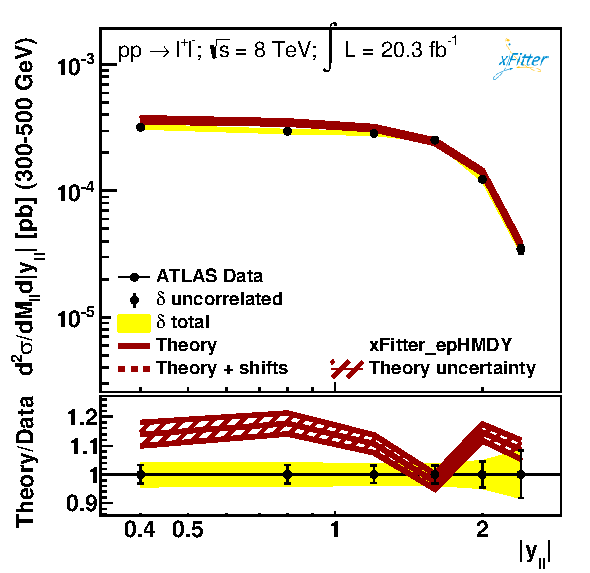
\includegraphics[width=7cm]{plots/data_4.pdf} 
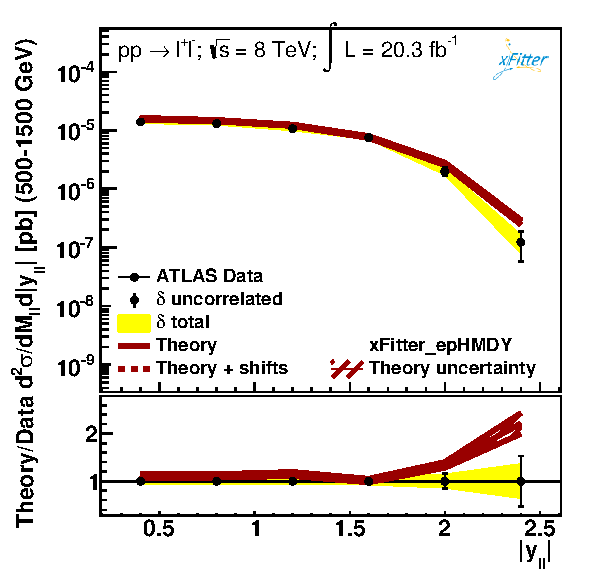
\includegraphics[width=7cm]{plots/data_5.pdf} 
\caption{Comparison between $\frac{d^{2}\sigma}{dm_{ll}d|y_{ll}|}$ for the high-mass Drell Yan data and the NNLo fit predictions.}
\label{hmDY_2D}
\end{figure}
The $\chi^{2}$ values for the high-mass Drell Yan data and the output parameters from NNLO fit can be found in Table.~\ref{chi2_scan} 
and Table.~\ref{par_scan} 
respectively. 
\begin{figure}
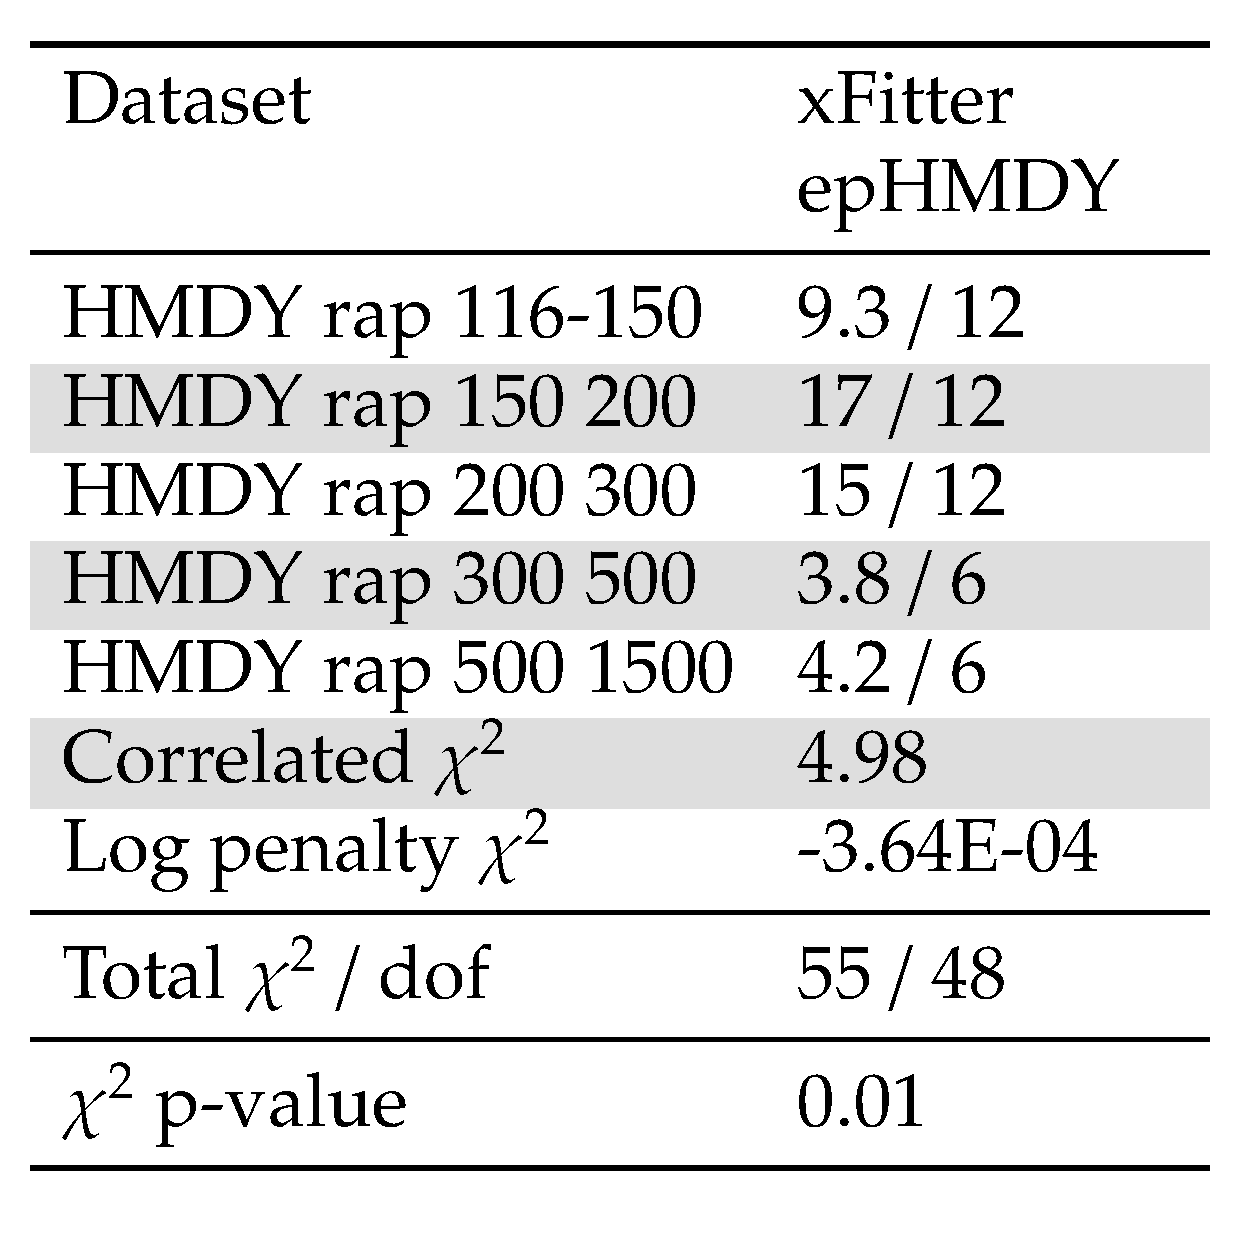
\includegraphics[width=14cm]{plots/chi2_hmDY.pdf} 
\caption{$\chi^{2}$ for high-mass Drell Yan data, for the NNLO fit}
\label{chi2_scan}
\end{figure}
\begin{figure}
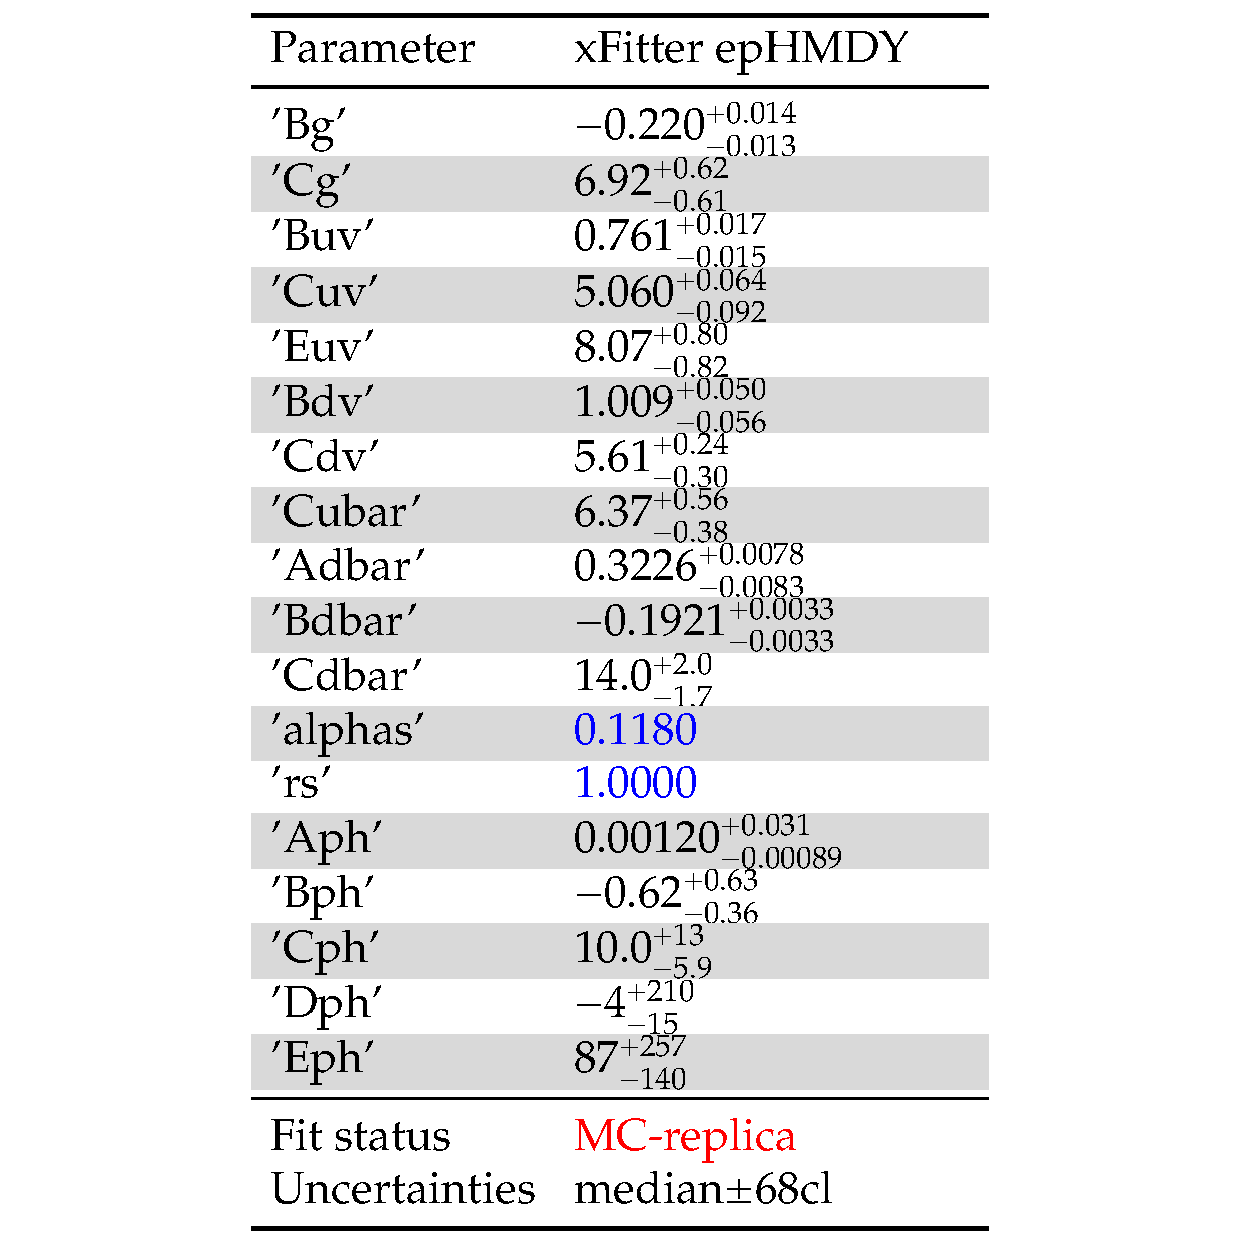
\includegraphics[width=14cm]{plots/parameters.pdf} 
\caption{PDF parameters for the NNLO fit.}
\label{par_scan}
\end{figure}

The NNLO photon PDF distribution is shown 
both at the starting scale (7.5 GeV$^{2}$) and at 10$^{4}$ GeV$^{2}$ 
 in Fig.~\ref{photon}, where it is also compared to an NLO extraction of the photon distribution.
The $x$-range of the figure is restricted to the range of sensitivity of the high-mass drell-Yan data;
$0.045 < x < 0.35$. The NLO and NNLO photon PDFs are compatible over this range.
\begin{figure}
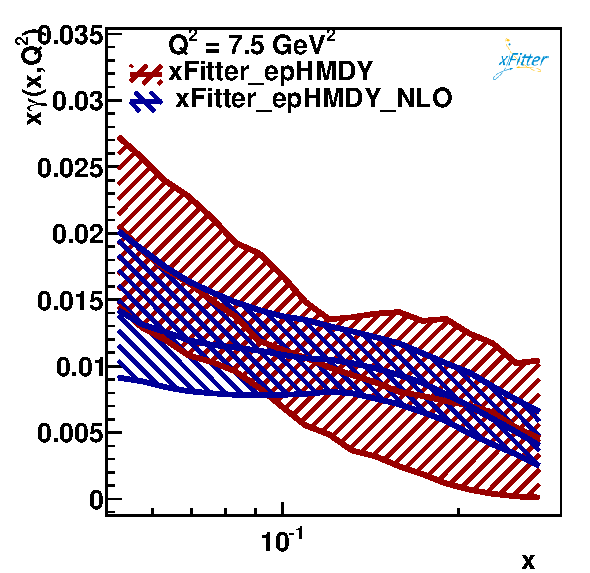
\includegraphics[width=7cm]{plots/photon_7_5.pdf} 
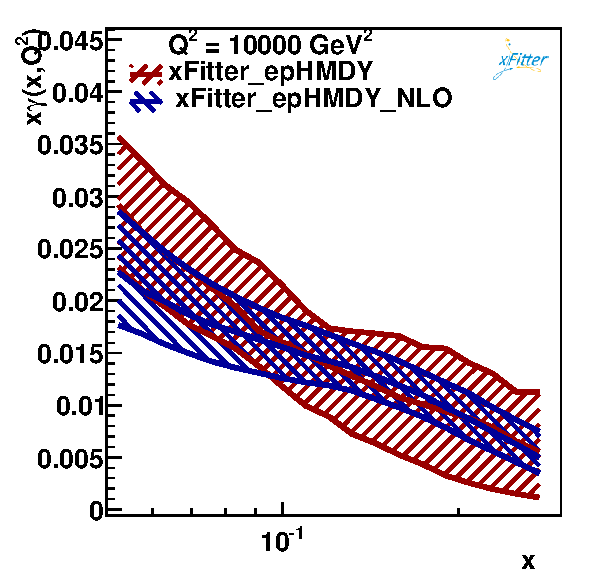
\includegraphics[width=7cm]{plots/photon_10000.pdf} 
\caption{Comparison between the photon PDF distributions at NNLO and NLO: (a) at the starting scale; (b) at the evolved scale.}
\label{photon}
\end{figure}

Fig.~\ref{photon_zoom} 
shows the photon distribution in the restricted range compared to the NNPDF3.0qed NNLO photon PDF.
The uncertainties are considerably reduced.
%
The comparison is shown at scale 100 GeV$^{2}$ and 
at 10$^{4}$ GeV$^{2}$, where the value of 100 GeV$^{2}$ is chosen such that comparisons can also be 
made to the LUXqed~\cite{Manohar:2016nzj}
photon PDF, which is only defined above this scale.
%
The 
HKR photon PDF~\cite{Harland-Lang:2016apc} is also shown in this figure.
%
The fit predictions from the present analysis
agree  with the LUXqed and the HKR photon PDFs at the 1-$\sigma$ level. 

\begin{figure}
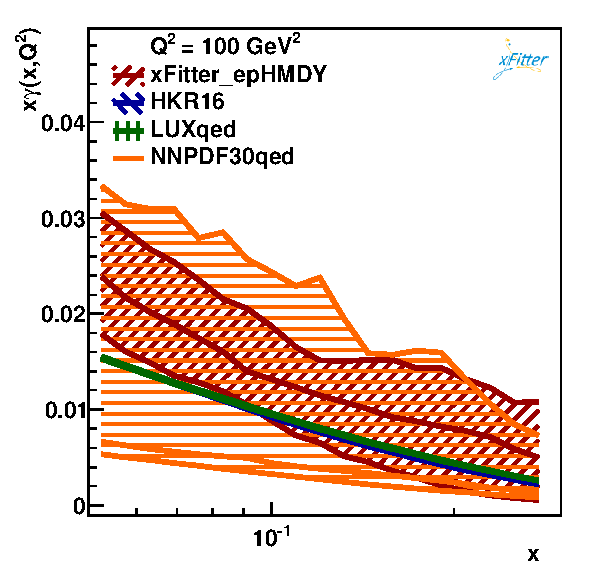
\includegraphics[width=7cm]{plots/photon_comp_100.pdf} 
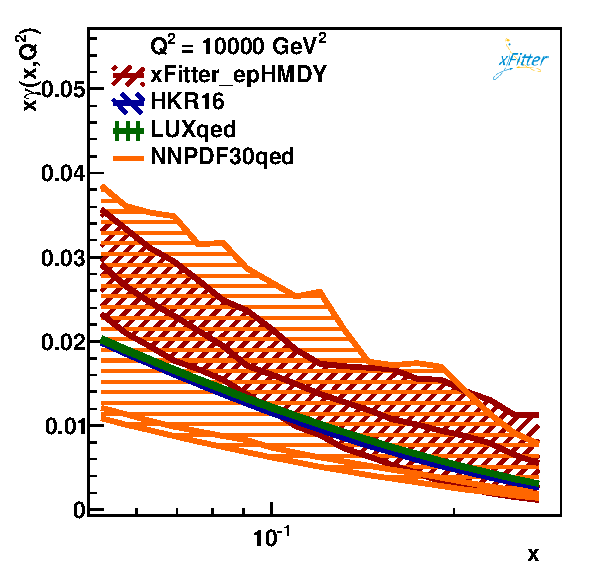
\includegraphics[width=7cm]{plots/photon_comp_10000.pdf} 
\caption{Comparison between the NNLO photon PDF distributions for the present analysis, NNPDF3.0QED, LUXqed, HKR: (a) at scale 100 GeV$^{2}$; (b) at the evolved scale 10000 GeV$^{2}$.}
\label{photon_zoom}
\end{figure}

